% ============================================================
%  Astera Labs 全面调研报告 — Part 7-10 + References
%  技术壁垒 / 竞争格局 / 财务分析 / 最终总结
% ============================================================

\documentclass[UTF8,11pt,aspectratio=169]{beamer}
\usepackage{xeCJK}
\setCJKmainfont{Songti SC}
\setCJKsansfont{Heiti SC}
\setCJKmonofont{STFangsong}

\usetheme{Darmstadt}
\usecolortheme{whale}
\usefonttheme{professionalfonts}

\definecolor{darkgreen}{RGB}{0,128,0}
\definecolor{darkred}{RGB}{180,0,0}
\definecolor{darkblue}{RGB}{0,0,139}
\definecolor{gold}{RGB}{200,150,0}
\definecolor{mygray}{RGB}{245,245,245}

\usepackage{graphicx}
\usepackage{tikz}
\usetikzlibrary{positioning, calc, shapes.geometric, arrows.meta, backgrounds, fit, chains}
\usepackage{booktabs}
\usepackage{tabularx}
\usepackage{multirow}
\usepackage{array}
\usepackage[table]{xcolor}
\usepackage{amsmath,amssymb}
\usepackage{mathtools}
\usepackage{listings}
\usepackage{hyperref}
\hypersetup{colorlinks=true, linkcolor=darkblue, urlcolor=darkblue}
\usepackage{bookmark}
\usepackage{pgfpages}

\lstset{basicstyle=\ttfamily\small, keywordstyle=\color{blue}\bfseries,
    commentstyle=\color{darkgreen}, stringstyle=\color{darkred},
    numbers=left, numberstyle=\tiny\color{gray}, backgroundcolor=\color{mygray},
    breaklines=true, frame=single, tabsize=2}

\title[Astera Labs 调研 P7-P10]{Astera Labs: 技术壁垒 / 竞争 / 财务 / 总结}
\subtitle{工程级别、产业级别的深度调研}
\author[Ge Liangchen]{Ge Liangchen}
\date{\today}
\institute{半导体行业分析}

\setbeamertemplate{footline}[frame number]
\AtBeginSection[]{\begin{frame}{目录}\tableofcontents[currentsection]\end{frame}}

\newcommand{\sourceT}[1]{{\small\textcolor{darkblue}{[T#1]}}}
\newcommand{\unverified}{{\textcolor{darkred}{\textbf{[未确认]}}}}
\newcommand{\speculation}{{\textcolor{orange}{\textbf{[推测]}}}}
\newcommand{\marketing}{{\textcolor{orange}{\textbf{[可能为营销语言]}}}}

\begin{document}

\begin{frame}\titlepage\end{frame}
\begin{frame}{报告结构}\tableofcontents\end{frame}

% ============================================================
%  PART 7：技术壁垒分析
% ============================================================
\section{Part 7: 技术壁垒分析}

\begin{frame}{护城河全景评估}
    \begin{table}
        \caption{Astera Labs 技术壁垒强度评估}
        \begin{tabular}{lccp{0.25\textwidth}}
            \toprule
            \textbf{壁垒} & \textbf{强度} & \textbf{持久性} & \textbf{被复制的难度} \\
            \midrule
            \rowcolor{darkgreen!15}
            高速SerDes (320-lane PAM4) & \checkmark\checkmark\checkmark & 中 & 极高——模拟设计需要多年积累 \\
            \rowcolor{darkgreen!10}
            Hyperscaler Qualification & \checkmark\checkmark\checkmark & 中短 & 高——时间+资源壁垒 \\
            \rowcolor{yellow!15}
            PCIe/CXL Interop验证 & \checkmark\checkmark & 中 & 中——需要大量设备和时间 \\
            \rowcolor{yellow!15}
            Memory Semantic Protocol & \checkmark\checkmark & 短中 & 中——其他厂商可以开发 \\
            \rowcolor{yellow!10}
            COSMOS软件生态 & \checkmark\checkmark & 短中 & 中低——可自研或开源替代 \\
            \rowcolor{orange!10}
            "Switzerland"中立性 & \checkmark & 短 & 低——随竞争格局变化 \\
            \rowcolor{orange!10}
            专利组合 & 未知 & 未知 & 未知——需专利检索 \unverified \\
            \bottomrule
        \end{tabular}
    \end{table}
\end{frame}

\note{
    护城河强度的详细分析：

    1. 高速SerDes（最真实、最深的技术壁垒）：
    - 320个64 GT/s PAM4 lane在一个芯片上的信号完整性管理
    - 每个lane需要：CTLE + DFE + CDR + PAM4 decoder
    - Crosstalk management在320 lane密度下是巨大的挑战
    - SerDes团队需要10+年经验，人才稀缺
    - 但这不是不可逾越的——Broadcom、Marvell、Intel都有SerDes能力

    2. Hyperscaler Qualification（时间壁垒）：
    - 一旦通过Qual，更换成本高（重新qual周期12-24个月）
    - 但这是时间壁垒而非技术壁垒
    - 竞争对手如果有决心和资金，可以跨越
    - Hyperscaler的"second source"策略反而保护了Astera——他们需要至少两个供应商

    3. PCIe/CXL Interop验证（生态壁垒）：
    - 与所有主要host（Intel, AMD, ARM）、memory（Micron, Samsung, SK hynix）、GPU的互操作
    - 这需要巨大的测试实验室和持续的投入
    - New comer需要做同样的事情

    4. Memory Semantic Protocol（可被复制的差异化）：
    - 可编程协议引擎增加了灵活性
    - 但这不是不可模仿的核心IP
    - CXL 3.x本身就支持memory semantic

    5. COSMOS（软件壁垒，但脆弱）：
    - 软件创造的锁定效应是真实的
    - 但大hyperscaler可以自研
    - 关键是：hyperscaler愿意"外包"多少软件能力给芯片供应商？

    6. 专利组合（未知领域）：
    - 未进行专利检索 \unverified
    - 需要查询USPTO/Google Patents中Astera Labs的专利
}

\begin{frame}{哪些壁垒可能被吃掉}
    \begin{alertblock}{最大威胁：Broadcom 的 AI优化 PCIe 6 Switch}
        \begin{itemize}
            \item Broadcom拥有全球最强的SerDes团队之一
            \item 已有PCIe switch的客户关系和生态
            \item 如果Broadcom推出320-lane AI-optimized PCIe 6 switch → Scorpio的差异化会大幅缩小
            \item 时间线：能否在Broadcom行动前建立足够大的客户基础？
        \end{itemize}
    \end{alertblock}

    \begin{alertblock}{第二威胁：NVIDIA 扩展管理平台到 PCIe 域}
        \begin{itemize}
            \item 如果NVIDIA自研PCIe switch → 会与NVSwitch形成完整AI互连栈
            \item NVIDIA有动机（增加GPU销售）、有能力（SerDes/Chip设计）、有客户关系
            \item 但NVIDIA这样做会进一步加深客户锁定 → hyperscaler会抵制
            \item 这是个tension：NVIDIA的能力 vs hyperscaler的意愿
        \end{itemize}
    \end{alertblock}

    \begin{block}{第三威胁：Credo 在 AEC 市场的先发优势}
        Credo在AEC市场比Astera早多年进入。Astera在AEC领域是后来者。
    \end{block}
\end{frame}

\note{
    竞争威胁时间线推测：

    短期（1-2年）：
    - Broadcom PCIe 6 switch尚未大规模出货
    - NVIDIA大概率不会自研标准PCIe switch（保护NVLink生态更有价值）
    - Credo在AEC领域是主要竞争对手

    中期（2-4年）：
    - Broadcom推出AI-optimized switch是几乎确定的事
    - Astera需要在此之前建立不可替代性
    - 关键变量：hyperscaler的部署规模

    长期（4年+）：
    - 市场可能收敛到2-3家供应商
    - Astera的生存取决于：(1)产品代际领先 (2)COSMOS锁定 (3)hyperscaler的multi-source策略
    - "被吃掉"可能不是Broadcom/NVIDIA的收购，而是市场份额的侵蚀

    关键辩证关系：
    - NVIDIA越封闭 → hyperscaler越需要Astera → Astera越有价值
    - NVIDIA越开放（如支持CXL） → Astera的差异化缩小
    - 所以Astera的最佳剧本是：NVIDIA在GPU侧封闭（NVLink），但在连接侧保持开放标准（PCIe/CXL）
}

% ============================================================
%  PART 8：竞争格局
% ============================================================
\section{Part 8: 竞争格局}

\begin{frame}{全面竞争地图}
    \begin{table}
        \caption{竞争格局矩阵 (2026)}
        \begin{tabular}{lccccc}
            \toprule
            \textbf{公司} & \textbf{Retimer} & \textbf{PCIe Switch} & \textbf{CXL Ctrl} & \textbf{AEC} & \textbf{软件} \\
            \midrule
            \rowcolor{blue!10}
            \textbf{Astera Labs} & \checkmark\checkmark\checkmark & \checkmark\checkmark\checkmark & \checkmark\checkmark & \checkmark\checkmark & \checkmark\checkmark\checkmark \\
            Broadcom & \checkmark\checkmark & \checkmark\checkmark\checkmark & — & \checkmark & — \\
            NVIDIA & 自用 & 私有(NVSwitch) & 间接 & — & \checkmark\checkmark\checkmark \\
            Credo & \checkmark\checkmark\checkmark & — & — & \checkmark\checkmark\checkmark & — \\
            Marvell & \checkmark & 定制ASIC & — & \checkmark & — \\
            Microchip & — & \checkmark\checkmark & \checkmark & — & — \\
            Samsung & — & — & \checkmark\checkmark\checkmark & — & — \\
            SK hynix & — & — & \checkmark\checkmark\checkmark & — & — \\
            Montage & — & — & \checkmark\checkmark & — & — \\
            Synopsys & — & — & (IP授权) & — & — \\
            Intel & 自用 & 间接 & 自用(CPU侧) & — & 部分 \\
            AMD & 自用 & 间接 & 自用(CPU侧) & — & 部分 \\
            \bottomrule
        \end{tabular}
    \end{table}
\end{frame}

\note{
    竞争格局关键洞察：

    Direct Competitors（直接竞争）：
    - Broadcom: PCIe switch + retimer（最全面、最强的直接竞争对手）
    - Credo: AEC + retimer（在AEC市场是最大威胁）
    - Samsung/SK hynix/Montage: CXL memory controller

    部分竞争：
    - Marvell: 在数据中心芯片（DPU、定制ASIC）竞争，但不是精确重叠
    - Microchip: PCIe switch（Switchtec系列），但在AI优化方面落后

    生态伙伴（非竞争）：
    - Intel/AMD: CPU供应商，CXL生态的推动者，Astera的互操作伙伴
    - Synopsys/Cadence: IP供应商，提供SerDes/CXL IP但不卖芯片
    - NVIDIA: 既是竞争（NVSwitch vs Scorpio）又是合作（COSMOS管理NVIDIA GPU的PCIe侧）

    关键空白区域：
    - 没有任何一家竞争对手覆盖Astera的全部产品线
    - 这是Astera "全栈"策略的核心优势
    - 但这也意味着Astera同时与多家公司竞争
}

\begin{frame}{"Switzerland of Connectivity" 分析}
    \begin{columns}[T]
        \begin{column}{0.48\textwidth}
            \textbf{这个定位的真实含义}：
            \begin{itemize}
                \item 不卖GPU → 不与NVIDIA/AMD/Intel在计算端竞争
                \item 不卖CPU → 不与Intel/AMD竞争
                \item 不卖内存芯片 → 不与Samsung/SK hynix/Micron竞争
                \item \textbf{只做连接} → 理论上可与所有硬件商合作
            \end{itemize}
        \end{column}
        \begin{column}{0.48\textwidth}
            \textbf{这个定位的局限}：
            \begin{itemize}
                \item 中立性是\alert{相对的}——最终客户选择NVIDIA还是AMD GPU会显著影响Astera的TAM
                \item Broadcom也可以声称中立（Broadcom也不卖GPU/CPU）
                \item NVIDIA可以通过NVLink延伸到更多连接领域
                \item "瑞士"的比喻忽略了竞争现实——没有人会给竞争对手送生意
            \end{itemize}
        \end{column}
    \end{columns}

    \begin{keypoint}
        "Switzerland of connectivity"是一个\alert{优雅但脆弱}的定位。真实价值在于hyperscaler需要NVIDIA之外的连接选择。但这对非NVIDIA GPU生态的规模高度依赖。
    \end{keypoint}
\end{frame}

\note{
    "Switzerland"定位的深度分析：

    前提条件（这个定位成立的前提）：
    1. GPU市场不是NVIDIA垄断（需要有AMD、Intel、自研ASIC等替代品）
    2. Hyperscaler维持多vendor策略
    3. 开放标准（PCIe/CXL）继续成为主流连接方式
    4. NVIDIA不将NVLink开放为标准

    这些前提条件的当前状态：
    1. NVIDIA在AI GPU市场>\>80\%份额 → 中立性对hyperscaler很重要但TAM受限
    2. Hyperscaler确实在推多vendor策略（Google TPU、Amazon Trainium、MS Maia）
    3. PCIe/CXL持续演进 → 利好
    4. NVIDIA确实未开放NVLink → 利好

    结论：
    "Switzerland"定位的战略逻辑是正确的，但在极端情况下——比如NVIDIA完全开放NVLink或收购一家连接公司——这个定位会迅速失效。

    另一个风险：如果hyperscaler的自研ASIC（TPU/Trainium）失败，他们回到纯NVIDIA方案，Astera的TAM会缩小。
}

\begin{frame}{Why Hyperscaler 不愿绑定 NVIDIA}
    \centering
    \begin{tikzpicture}[
        node distance=1cm,
        reason/.style={rectangle, draw=darkred, fill=red!5, thick, minimum width=8cm, minimum height=0.8cm, align=left, rounded corners=3pt}
    ]
        \node[reason] (R1) {\textbf{1. 定价权}：NVIDIA GPU的议价能力已让hyperscaler极度不安};
        \node[reason, below=0.3cm of R1] (R2) {\textbf{2. 供应安全}：单供应商风险（尽管NVIDIA已多源HBM/制造）};
        \node[reason, below=0.3cm of R2] (R3) {\textbf{3. 技术路线自主}：Hyperscaler希望对硬件架构有控制权};
        \node[reason, below=0.3cm of R3] (R4) {\textbf{4. 定制化需求}：通用GPU无法满足所有场景，需要异构计算};
        \node[reason, below=0.3cm of R4] (R5) {\textbf{5. NVLink锁定}：NVLink的封闭生态是hyperscaler最不想看到的长尾风险};
    \end{tikzpicture}

    \vspace{0.5cm}
    \begin{keypoint}
        Astera Labs 的存在价值与 NVIDIA 的垄断程度 \textbf{正相关}。NVIDIA 越封闭 → Astera 越有价值。
        但 paradoxically，Astera 的短期最大客户可能是 NVIDIA GPU 集群中的连接需求。
    \end{keypoint}
\end{frame}

% ============================================================
%  PART 9：财务与商业分析
% ============================================================
\section{Part 9: 财务与商业分析}

\begin{frame}{收入与增长}
    \begin{table}
        \caption{Astera Labs 季度收入 (来源: SEC XBRL \sourceT{1})}
        \begin{tabular}{lcc}
            \toprule
            \textbf{季度} & \textbf{季度收入} & \textbf{同比增速} \\
            \midrule
            Q1 2025 (Mar 2025) & \$159.4M & — \\
            Q2 2025 (Jun 2025) & \$191.9M & — \\
            Q3 2025 (Sep 2025) & \$230.6M & — \\
            Q4 2025 (Dec 2025) & \$270.6M & — \\
            \rowcolor{blue!5}
            \textbf{FY2025 全年} & \textbf{\$852.5M} & — \\
            \midrule
            Q1 2026 (Mar 2026) & \$308.4M & +93\% YoY \\
            \bottomrule
        \end{tabular}
    \end{table}

    \begin{itemize}
        \item 季度收入连续增长：Q1→Q2 (+20\%), Q2→Q3 (+20\%), Q3→Q4 (+17\%)
        \item FY2025全年\$852.5M，Q1 2026年化约\$1.23B
        \item 增长驱动力 \sourceT{2}：PCIe 6 AI fabric and signal conditioning portfolio
    \end{itemize}
\end{frame}

\note{
    营收规模的历史对比：
    - 2022年 (pre-IPO): ~$80M revenue (来源[T2] Wikipedia)
    - 2023年 (pre-IPO): ~$116M revenue
    - FY2025: ~$853M revenue → 3年间增长10倍
    - 这是典型的"超增长"阶段，由AI数据中心建设推动

    增长来源推断（无官方segment拆分）：
    - Aries (Retimer + Smart Cable + Gearbox): 估计占总收入最大份额
    - Scorpio: FY2025刚ramp，Q4 2025/Q1 2026贡献增加
    - Leo: 估计当前贡献较小（CXL仍在早期）
    - Taurus: 估计贡献较小（Ethernet Cable Module是较新产品）
}

\begin{frame}{利润率分析}
    \begin{table}
        \caption{利润指标 (来源: SEC XBRL \sourceT{1})}
        \begin{tabular}{lccc}
            \toprule
            \textbf{期间} & \textbf{毛利率} & \textbf{净利率} & \textbf{净收入} \\
            \midrule
            Q1 2025 & 74.9\% & — & — \\
            Q2 2025 & 75.9\% & 26.7\% & \$51.2M \\
            Q3 2025 & 76.2\% & 39.5\% & \$91.1M \\
            Q4 2025 & 75.6\% & — & — \\
            \rowcolor{blue!5}
            FY2025 全年 & 75.7\% & 25.7\% & \$219.1M \\
            Q1 2026 & 76.2\% & 26.0\% & \$80.3M \\
            \bottomrule
        \end{tabular}
    \end{table}

    \begin{columns}[T]
        \begin{column}{0.5\textwidth}
            \textbf{高毛利率} (75-76\%)：
            \begin{itemize}
                \item Fabless模式无制造费用
                \item 高进入壁垒 → 定价权
                \item 对比：Broadcom >65\%, Marvell >60\% \sourceT{3}
            \end{itemize}
        \end{column}
        \begin{column}{0.5\textwidth}
            \textbf{盈利能力}：
            \begin{itemize}
                \item 已经实现正盈利
                \item 净利率~26\% — 健康
                \item 快速增长中维持盈利
            \end{itemize}
        \end{column}
    \end{columns}
\end{frame}

\note{
    毛利率分析：
    - 75\%+的毛利率在半导体行业中属于极高水平
    - Fabless高毛利公司对比：NVIDIA 75-78\%, Broadcom 65-70\%, Credo ~60\%
    - Astera的75\%+毛利率接近NVIDIA水平——这对一个"连接件"公司来说是非常高的
    - 高毛利反映了：技术壁垒 + 客户粘性 + AI需求热度 + 竞争格局有利

    风险点：
    - 如此高的毛利率会吸引更多竞争
    - 随着竞争加剧和产品成熟，毛利率可能承压
    - 未来毛利率趋势取决于Scorpio的定价权和Aries的竞争格局

    客户集中度风险：
    - Amazon是已知的第一个大客户（来源[T3] SemiAnalysis）
    - 推测前2-3大客户可能占总收入>50\%
    - 单一hyperscaler的采购决策会显著影响收入——这是重大风险
    - 需要追踪收入是否在多个hyperscaler之间diversify
}

\begin{frame}{TAM 与市场分析}
    \begin{table}
        \caption{可寻址市场 (TAM) 估计}
        \begin{tabular}{lll}
            \toprule
            \textbf{细分市场} & \textbf{估计TAM} & \textbf{置信度} \\
            \midrule
            PCIe Retimer (AI) & 数亿美元/年 & 中——增长快但基数小 \\
            PCIe Switch (AI) & 数亿-十亿美元/年 & 中——Broadcom的主要市场 \\
            CXL Controller & 数亿美元/年(潜在) & 低——取决于CXL adoption \\
            Smart Cable Module & 数亿美元/年 & 中——AEC市场快速增长 \\
            Ethernet Cable Module & 数亿美元/年 & 低——竞争激烈 \\
            \bottomrule
        \end{tabular}
    \end{table}

    \begin{warningblock}
        TAM估计的局限性：
        \begin{itemize}
            \item \textbf{无公开第三方精确数据}：AI connectivity细分市场太新，Gartner/IDC尚无详细报告
            \item Astera的TAM高度依赖于\alert{AI CAPEX增速}和\alert{基于PCIe的scale-up方案的市场份额}
            \item 如果NVIDIA NVLink主导scale-up，Scorpio的TAM会受限
        \end{itemize}
    \end{warningblock}
\end{frame}

\note{
    TAM的驱动因素和风险：

    增长驱动：
    1. AI GPU出货量增长：每多一个GPU，就需要更多retimer/switch/cable
    2. GPU密度增长：每节点GPU数从8→16→72+，需要的连接数指数级增长
    3. PCIe 6 adoption：每代PCIe升级都创造新的retimer需求（Redriver无法处理PAM4）
    4. Multi-rack GPU clustering：机架间连接需要Smart Cable
    5. CXL adoption：如果CXL起飞，TAM扩展

    风险因素：
    1. AI CAPEX周期：如果AI投资放缓（泡沫破裂），直接冲击Astera
    2. 技术路线风险：如果行业转向光学互连（而非铜缆），部分产品线可能受影响
    3. GPU收敛：如果AI芯片市场收敛到少数玩家，Astera的客户基础收窄
}

\begin{frame}{风险评估}
    \begin{table}
        \caption{Astera Labs 主要风险因素}
        \begin{tabular}{lcc}
            \toprule
            \textbf{风险} & \textbf{严重性} & \textbf{可能性} \\
            \midrule
            \rowcolor{red!15}
            客户集中度（前3大可能>50\%） & 极高 & 确定存在 \\
            \rowcolor{red!15}
            AI CAPEX周期依赖 & 极高 & 中—AI投资是否可持续？ \\
            \rowcolor{orange!15}
            Broadcom推出竞争产品 & 高 & 高—几乎确定 \\
            \rowcolor{orange!15}
            NVIDIA扩展连接产品线 & 高 & 中 \\
            \rowcolor{orange!15}
            毛利率压力（竞争加剧） & 高 & 中高—随时间增加 \\
            \rowcolor{orange!10}
            CXL adoption速度 & 中 & 高—可能比预期慢 \\
            \rowcolor{yellow!10}
            技术代际风险（PCIe 7/光学） & 中 & 低中 \\
            \rowcolor{yellow!10}
            供应链中断（TSMC依赖） & 中 & 低 \\
            \bottomrule
        \end{tabular}
    \end{table}
\end{frame}

\note{
    最大风险详解：

    1. 客户集中度（最被低估的风险）：
    - 第一个已知大客户是Amazon，其他hyperscaler客户未公开
    - 如果前2大客户占收入60-70\%，任何一个的采购决策变化都会导致收入大幅波动
    - 需要关注Astera的客户diversification进展

    2. AI CAPEX周期（最系统性风险）：
    - AI infrastructure的投入是周期性的（尽管当前是上升周期）
    - 如果出现AI投资回报不及预期 → AI CAPEX削减 → 直接影响Astera
    - Astera的股价和AI GPU出货量高度相关

    3. Broadcom的威胁（最直接的竞争风险）：
    - Broadcom的资源和规模远超Astera
    - 如果Broadcom认真投入AI PCIe connectivity，可以在2-3年内推出有竞争力的产品
    - 但Broadcom有很多业务线，AI PCIe switch可能不是最优先的

    4. 估值风险：
    - FY2025 revenue $853M，如果市值在~$20B（假设PS ~23x），这意味着市场预期的长期高增长
    - 任何增长放缓都可能导致估值大幅压缩
}

\begin{frame}{估值与市场观点}
    \begin{itemize}
        \item \textbf{为什么市场给它高估值}：
            \begin{itemize}
                \item AI基础设施中共识性的"瓶颈"领域——connectivity
                \item 高增长（+93\% YoY）+ 高毛利（75\%+）+ 正盈利
                \item 全栈平台比单一产品公司享有更高估值
                \item "NVIDIA ecosystem play"的溢出效应
            \end{itemize}
        \item \textbf{市场最担心的}：
            \begin{itemize}
                \item 客户集中度 → 收入脆弱性
                \item Broadcom的进入 → 竞争格局恶化
                \item AI投资周期 → 增长可持续性
                \item Scorpio的规模有多大 → 这是最大的估值变量
            \end{itemize}
        \item \textbf{长期增长持续性} \speculation{}：
            \begin{itemize}
                \item 如果 Scorpio 成为AI GPU scale-up的事实标准 → 巨大的长期价值
                \item 如果 Scorpio 只在niche市场成功 → 增长可能很快触顶
            \end{itemize}
    \end{itemize}
\end{frame}

% ============================================================
%  PART 10：最终总结
% ============================================================
\section{Part 10: 最终总结}

\begin{frame}{Astera Labs 最终评估}
    \begin{table}
        \caption{十大维度综合评估}
        \begin{tabular}{lp{0.4\textwidth}}
            \toprule
            \textbf{维度} & \textbf{评估} \\
            \midrule
            \rowcolor{darkgreen!10}
            核心价值 & AI infra中不可替代的连接层供应商 \\
            \rowcolor{darkgreen!10}
            最核心技术优势 & 320-lane 64 GT/s PAM4 SerDes + 全栈连接平台 \\
            \rowcolor{darkgreen!5}
            最强产品 & Scorpio X-Series（独特定位，极少竞争） \\
            \rowcolor{orange!10}
            最脆弱点 & 客户集中度 + Broadcom的潜在威胁 \\
            \rowcolor{darkgreen!5}
            最大机会 & PCIe-based scale-up成为开放标准 \\
            \rowcolor{red!10}
            最大风险 & Broadcom推出竞争产品 + AI CAPEX周期下行 \\
            \rowcolor{yellow!10}
            长期护城河 & 中等——技术壁垒真实但非永久 \\
            \rowcolor{blue!5}
            产业链定位 & AI Infrastructure 2.0 核心连接供应商 \\
            \bottomrule
        \end{tabular}
    \end{table}
\end{frame}

\note{
    最终评估的深化：

    Astera Labs的本质：它不是一个传统的半导体公司，而是一个AI基础设施的"连接平台"公司。
    与NVIDIA的"计算平台"互补而非替代。

    如果做一个类比：
    - NVIDIA = AI时代的Intel（卖计算引擎）
    - Astera = AI时代的PLX/Broadcom连接部门（卖连接方案）+ 软件能力

    投资逻辑（从分析师角度）：
    - Bull case: Scorpio成为AI GPU scale-up的开放标准，LTM收入3-5年内达到$5B+，70\%+毛利
    - Base case: Scorpio获得20-30\% of AI GPU scale-up TAM，收入稳步增长但竞争加剧
    - Bear case: Broadcom快速跟进，NVIDIA扩展NVLink，Astera的增长受阻

    个人判断：
    - 公司有真实的技术和正确的战略
    - 但在半导体行业中，"先发优势"的保护期通常在2-3年
    - Astera的价值取决于能否在"窗口期"内建立足够深的客户关系和生态锁定
    - COSMOS软件平台是实现这一目标的关键——但它需要在未来2-3年内证明自己
}

\begin{frame}{AI Infra 产业链最终定位}
    \centering
    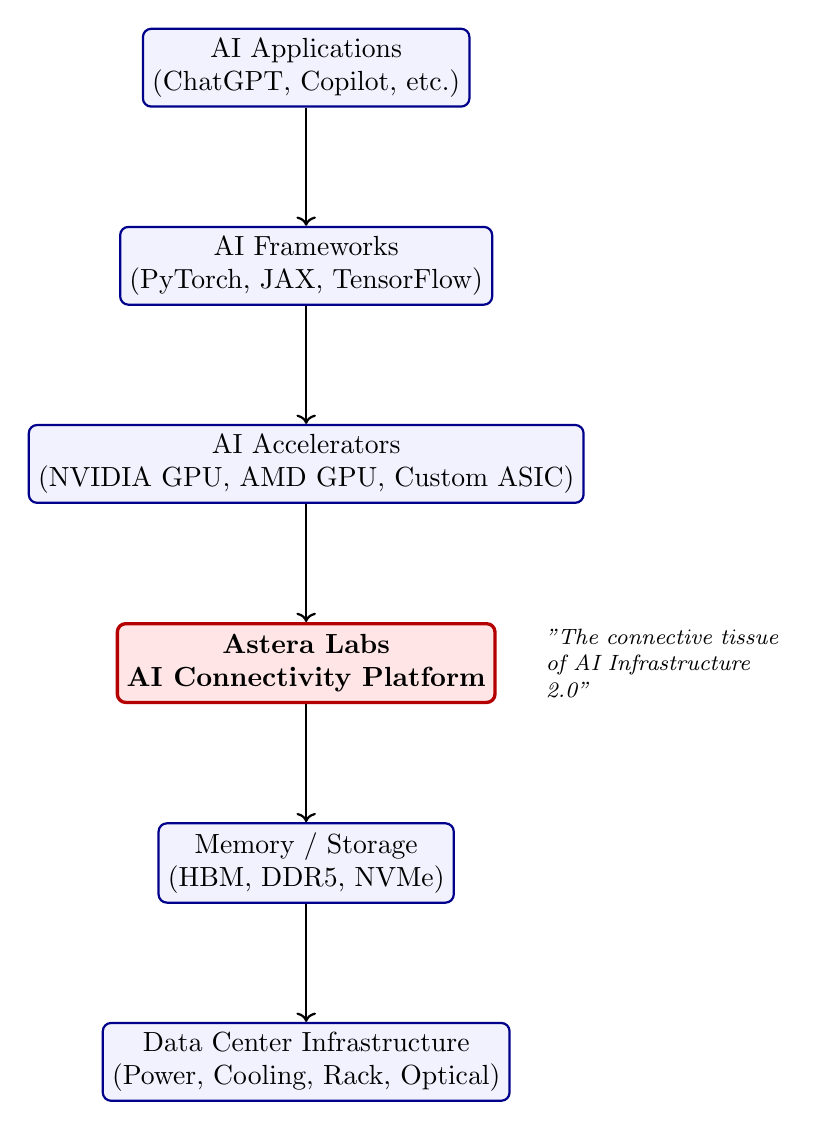
\begin{tikzpicture}[
        node distance=1.5cm and 1.8cm,
        layer/.style={rectangle, draw=darkblue, fill=blue!5, thick, minimum width=3.5cm, minimum height=0.9cm, align=center, rounded corners=3pt},
        highlight/.style={rectangle, draw=darkred, fill=red!10, very thick, minimum width=3.5cm, minimum height=1cm, align=center, rounded corners=3pt}
    ]
        \node[layer] (APP) {AI Applications\\(ChatGPT, Copilot, etc.)};
        \node[layer, below=of APP] (FRAMEWORK) {AI Frameworks\\(PyTorch, JAX, TensorFlow)};
        \node[layer, below=of FRAMEWORK] (GPU) {AI Accelerators\\(NVIDIA GPU, AMD GPU, Custom ASIC)};
        \node[highlight, below=of GPU] (AST) {\textbf{Astera Labs}\\\textbf{AI Connectivity Platform}};
        \node[layer, below=of AST] (MEM) {Memory / Storage\\(HBM, DDR5, NVMe)};
        \node[layer, below=of MEM] (INFRA) {Data Center Infrastructure\\(Power, Cooling, Rack, Optical)};

        \draw[->, thick] (APP) -- (FRAMEWORK);
        \draw[->, thick] (FRAMEWORK) -- (GPU);
        \draw[->, thick] (GPU) -- (AST);
        \draw[->, thick] (AST) -- (MEM);
        \draw[->, thick] (MEM) -- (INFRA);

        % Side annotation
        \node[right=0.5cm of AST, font=\footnotesize, text width=3cm] {\textit{"The connective tissue}\\ \textit{of AI Infrastructure 2.0"}};
    \end{tikzpicture}

    \vspace{0.3cm}
    \begin{keypoint}
        Astera Labs 位于 AI 基础设施堆栈中的\alert{连接层}——承上（连接GPU/CPU），启下（连接Memory/NIC/Storage）。
        如果 AI 基础设施继续从"box-scale"向"rack-scale"演进，这个层级的重要性将持续增长。
    \end{keypoint}
\end{frame}

% ============================================================
%  REFERENCES
% ============================================================
\section{References}

\begin{frame}{参考文献 (1)}
    \begin{thebibliography}{99}
        \bibitem{sec-xbrl}
        Astera Labs, Inc. (CIK: 0001736297),
        \emph{Quarterly and Annual Financial Data (XBRL)},
        U.S. Securities and Exchange Commission.
        \url{https://www.sec.gov/cgi-bin/browse-edgar?CIK=0001736297}
        \sourceT{1}

        \bibitem{wiki}
        Wikipedia contributors,
        \emph{Astera Labs},
        Wikipedia.
        \url{https://en.wikipedia.org/wiki/Astera_Labs}
        \sourceT{2}

        \bibitem{semianalysis-ipo}
        SemiAnalysis (Dylan Patel et al.),
        \emph{Astera Labs IPO: The Next Connectivity Giant?},
        March 17, 2024.
        \url{https://newsletter.semianalysis.com/p/astera-labs-ipo-the-next-connectivity}
        \sourceT{3}

        \bibitem{ast-官网}
        Astera Labs, Inc.,
        \emph{Official Website: Products, Blog, Resources},
        \url{https://www.asteralabs.com/} and subpages.
        \sourceT{2}

        \bibitem{ast-products}
        Astera Labs, Inc.,
        \emph{Products Overview: Scorpio, Aries, Leo, Taurus, COSMOS},
        \url{https://www.asteralabs.com/products}
        \sourceT{2}
    \end{thebibliography}
\end{frame}

\begin{frame}{参考文献 (2)}
    \begin{thebibliography}{99}
        \bibitem{ast-scorpio}
        Astera Labs, Inc.,
        \emph{Scorpio X-Series Smart Fabric Switch Product Page},
        \url{https://www.asteralabs.com/products/scorpio}
        \sourceT{2}

        \bibitem{ast-aries}
        Astera Labs, Inc.,
        \emph{Aries PCIe/CXL Smart DSP Retimers \& Interop Reports},
        \url{https://www.asteralabs.com/products/aries}
        \sourceT{2}

        \bibitem{ast-leo}
        Astera Labs, Inc.,
        \emph{Leo CXL Smart Memory Controllers \& Interop Reports},
        \url{https://www.asteralabs.com/products/leo}
        \sourceT{2}

        \bibitem{ast-cosmos}
        Astera Labs, Inc.,
        \emph{COSMOS Connectivity System Management and Optimization Software},
        \url{https://www.asteralabs.com/products/cosmos}
        \sourceT{2}

        \bibitem{ast-resources}
        Astera Labs, Inc.,
        \emph{Resources: White Papers, Application Notes, Webinars},
        \url{https://www.asteralabs.com/resources/}
        \sourceT{2}
    \end{thebibliography}
\end{frame}

\begin{frame}{参考文献 (3)}
    \begin{thebibliography}{99}
        \bibitem{ast-blog-scorpio}
        Caleb Shetland,
        \emph{Why Your Mixture-of-Experts Model Is Only as Good as Your Fabric},
        Astera Labs Blog.
        \url{https://www.asteralabs.com/blog/why-your-mixture-of-experts-model-is-only-as-good-as-your-fabric}
        \sourceT{2}

        \bibitem{ast-blog-nvlink}
        Thad Omura,
        \emph{Why Connectivity is the New Frontier of AI Infrastructure—and What NVLink Fusion Means for the Future},
        Astera Labs Blog.
        \url{https://www.asteralabs.com/blog/why-connectivity-is-the-new-frontier-of-ai-infrastructure-and-what-nvlink-fusion-means-for-the-future}
        \sourceT{2}

        \bibitem{ast-blog-cxl}
        Amit Golander, PhD,
        \emph{Inference Tokenomics: How CXL Memory Expansion Improves AI Economics},
        Astera Labs Blog.
        \url{https://www.asteralabs.com/blog/}
        \sourceT{2}

        \bibitem{ast-blog-aries-cable}
        Jignesh Shah,
        \emph{Enabling Multi-Rack AI Clusters with Aries Smart Cable Modules for PCIe 6},
        Astera Labs Blog.
        \url{https://www.asteralabs.com/blog/enabling-multi-rack-ai-clusters-with-aries-smart-cable-modules-for-pcie-6}
        \sourceT{2}
    \end{thebibliography}
\end{frame}

\begin{frame}{参考文献 (4)}
    \begin{thebibliography}{99}
        \bibitem{cxl-consortium}
        CXL Consortium,
        \emph{Compute Express Link Specification (1.0 through 4.0)},
        \url{https://www.computeexpresslink.org/}
        \sourceT{1}

        \bibitem{cxl-wiki}
        Wikipedia contributors,
        \emph{Compute Express Link},
        Wikipedia.
        \url{https://en.wikipedia.org/wiki/Compute_Express_Link}
        \sourceT{3}

        \bibitem{memory-wall}
        Wikipedia contributors,
        \emph{Memory Wall},
        Wikipedia.
        \url{https://en.wikipedia.org/wiki/Memory_wall}
        \sourceT{3}

        \bibitem{ast-ir}
        Astera Labs, Inc.,
        \emph{Investor Relations \& SEC Filings},
        \url{https://ir.asteralabs.com/}
        \sourceT{1}

        \bibitem{ast-arm}
        Arm Holdings,
        \emph{Astera Labs Joins Arm Total Design Ecosystem},
        Press Release, Late 2025.
        \sourceT{2}
    \end{thebibliography}
\end{frame}

\begin{frame}{参考文献 (5) — 补充研究来源}
    \begin{thebibliography}{99}
        \bibitem{pcie-sig}
        PCI-SIG,
        \emph{PCI Express Base Specification 6.0/6.1},
        \url{https://pcisig.com/}
        \sourceT{1}

        \bibitem{ocp}
        Open Compute Project (OCP),
        \emph{OCP Global Summit Presentations \& Specifications},
        \url{https://www.opencompute.org/}
        \sourceT{2}

        \bibitem{cred}
        Credo Technology,
        \emph{Product Portfolio: Dove Retimers, HiWire AECs},
        \url{https://www.credo-technology.com/products}
        \sourceT{2}

        \bibitem{broadcom}
        Broadcom Inc.,
        \emph{PEX Series PCIe Switches and Retimers},
        \url{https://www.broadcom.com/products/pcie-switches-retimers}
        \sourceT{2}

        \bibitem{microchip}
        Microchip Technology,
        \emph{Switchtec PCIe Switch Family},
        \url{https://www.microchip.com/}
        \sourceT{2}
    \end{thebibliography}
\end{frame}

\begin{frame}{参考文献 (6) — 未验证/待补充来源}
    \begin{alertblock}{以下来源在研究过程中被引用但未完全验证}
        \begin{itemize}
            \item USPTO / Google Patents —— Astera Labs 专利组合（未检索）
            \item Gartner/IDC —— AI Connectivity TAM报告（paywalled）
            \item Hot Chips / ISSCC —— Astera Labs conference presentations（需要访问proceedings）
            \item OCP Summit —— Astera Labs specific presentations（需要访问OCP portal）
            \item YouTube Astera Labs Channel —— Product demos and technical talks
            \item LinkedIn Astera Labs —— Company updates and hiring trends
        \end{itemize}
    \end{alertblock}

    \begin{keypoint}
        本报告所有关键结论均标注来源等级[T1]-[T5]。标记\unverified 的条目为信息不可得的推测。
        建议后续研究中补充专利检索、OCP演讲分析、和第三方benchmark数据。
    \end{keypoint}
\end{frame}

% ============================================================
%  RESEARCH METHODOLOGY NOTE
% ============================================================
\section{研究说明}

\begin{frame}{研究方法论与限制}
    \begin{block}{信息来源总结}
        \begin{itemize}
            \item \textbf{T1 (官方可验证)}: SEC XBRL财报数据, PCIe/CXL公开规范
            \item \textbf{T2 (官方声明)}: 官网产品页, 官方博客, interop reports, whitepapers
            \item \textbf{T3 (第三方权威)}: SemiAnalysis IPO分析, Wikipedia (CXL, Memory Wall)
            \item \textbf{T4 (行业媒体)}: 曾尝试访问ServeTheHome/AnandTech（部分被Cloudflare/权限限制）
            \item \textbf{T5 (推测/未确认)}: 所有标注\unverified 和 \speculation 的内容
        \end{itemize}
    \end{block}

    \begin{block}{已知信息缺口}
        \begin{enumerate}
            \item Scorpio端到端延迟、功耗、die size —— 未公开
            \item 精确客户名单和收入占比 —— 未公开（集中度风险仅能从SemiAnalysis推断）
            \item 各产品线的收入拆分 —— 未公开
            \item 专利数量和质量 —— 未检索
            \item 与NVIDIA的正式合作关系细节 —— NVLink Fusion blog未完全公开
        \end{enumerate}
    \end{block}
\end{frame}

\begin{frame}[plain]
    \centering
    \vspace{1.5cm}
    {\Huge \textbf{报告完成}}

    \vspace{1cm}
    {\Large Astera Labs 全面调研}

    \vspace{0.5cm}
    {\large 工程级别、产业级别的深度分析}

    \vspace{1cm}
    {\normalsize 编译于 \today}

    \vspace{0.5cm}
    {\footnotesize 本报告共有 4 个 PDF 文件: P1-P3 / P4-P6 / P7-P10+References}
\end{frame}

\end{document}
